\documentclass[rnd]{mas_proposal}
% \documentclass[thesis]{mas_proposal}

\usepackage[utf8]{inputenc}
\usepackage{amsmath}
\usepackage{amsfonts}
\usepackage{amssymb}
\usepackage{graphicx}

\title{Project Proposal Title}
\author{First Name Last Name}
\supervisors{First Supervisor\\Second Supervisor\\Third Supervisor}
\date{Month 20XX}

% \thirdpartylogo{path/to/your/image}

\begin{document}

\maketitle

\pagestyle{plain}

\section{Introduction}

\subsection{Topic of This R\&D Project}
\begin{itemize}
    \item Provide reasonably detailed description of what you intent to do in your R\&D project.
    \item You may also discuss the challenges that you have to address.
    \item Reflect on the profile of the reader and PLEAAAASE, tell a story here and refrain from bombarding the readers with details which they may not be able to appreciate.
\end{itemize}

\subsection{Relevance of This R\&D Project}
\begin{itemize}
    \item Who will benefit from the results of this R\&D project?
    \item What are the benefits? Quantify the benefits with concrete numbers.
 \end{itemize}

\section{Related Work}

\subsection{Survey of Related Work}
\begin{itemize}
    \item What have other people done to solve the problem?
    \item You should reference and briefly discuss at least the ``top twelve'' related works
\end{itemize}

\subsection{Limitation and Deficits in the State of the Art}
\begin{itemize}
    \item List the deficits that you have discovered in the related work and explain them such that a person who is not deep into the technical details can still understand them.
    For each deficit, provide at least two references
    \item You should reference and briefly discuss at least the ``top twelve'' related works
\end{itemize}

\section{Problem Statement}
\begin{itemize}
    \item Which of the deficits are you going to solve?
    \item What is your intended approach?
    \item How will you compare you approach with existing approaches?
\end{itemize}

\section{Project Plan}

\subsection{Work Packages}
\emph{Planning is the replacement of randomness by error.} (Einstein). Very much like you would never start a longer journey without a detailed travel plan, you should not start a project without a carefully though out work plan. A work package is a logical decomposition of a larger piece of work into smaller parts following a ``divide and conquer" strategy. It is very specific to the problem that you are going to address. Refrain from a rather generic decomposition. If your work plan looks similar to those of your school mates, which may address completely different problems then you have not thought carefully enough about how you approach the problem. It is ok to have two generic work packages \emph{Literature Study} and \emph{Project Report}. Discuss your work packages in the ASW seminar.

The bare minimum will include the following packages:
\begin{enumerate}
    \item[WP1] Literature Study
    \item[WP2] ...
    \item[WP3] ...
    \item  ...
    \item[WPy] Evaluation of approach and comparison with similar approaches
    \item[WPz] Project Report
\end{enumerate}

\subsection{Milestones}
Milestones mark the completion of a certain activity or at least a major achievement in an activity. Milestones are also decision points, where you reflect on what you have achieved and what options you have for continuing your work in case you have not achieved what was planned. Above all, milestones have to be measurable. As above, if your milestones are the same as those of your school mates, then you may not have thought carefully enough about how your project shall progress.
\begin{enumerate}
    \item[M1] Literature review completed and best practice identified
    \item[M2] ...
    \item[M3] ...
    \item[M4] Report submission
\end{enumerate}

\subsection{Project Schedule}
Include a Gantt chart here. It doesn't have to be detailed, but it should include the milestones you mentioned above.
Make sure to include the writing of your report throughout the whole project, not just at the end.

\begin{figure}[h!]
    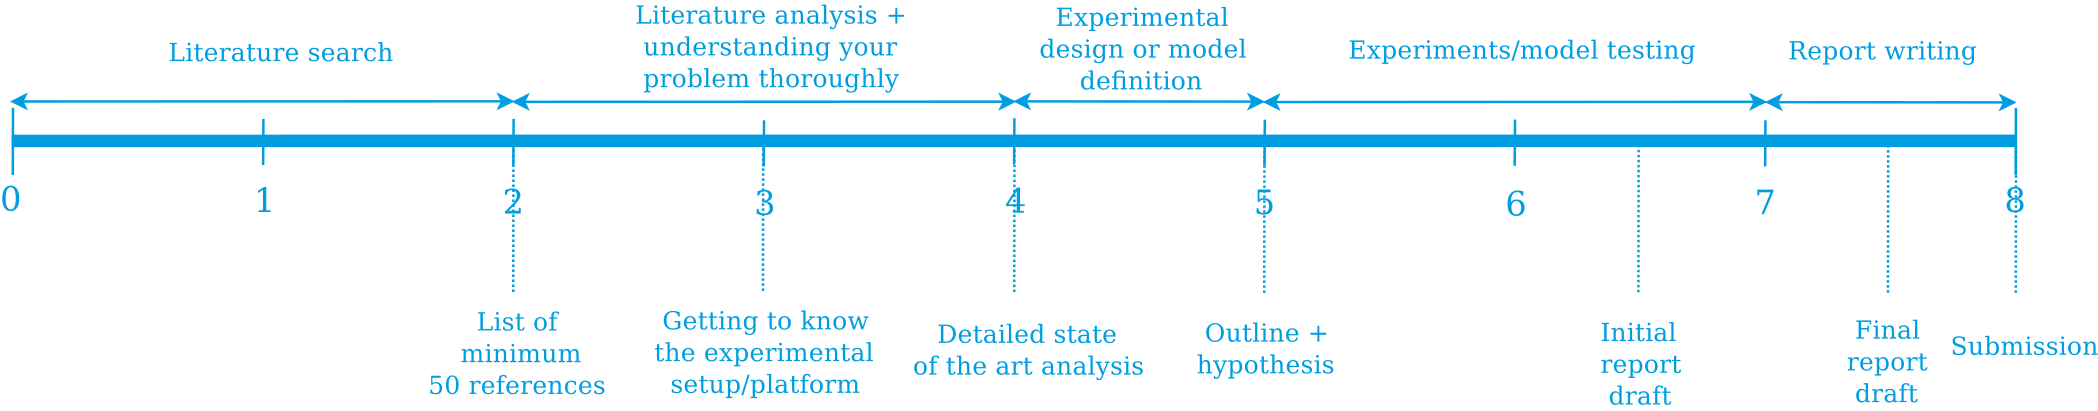
\includegraphics[width=\textwidth]{images/rnd_deliverable_timeline}
    \caption{My figure caption}
    \label{fig:myfigure}
\end{figure}

\subsection{Deliverables}

\subsubsection*{Minimum Viable}
\begin{itemize}
    \item Project results required to get a satisfying or sufficient grade.
\end{itemize}

\subsubsection*{Expected}
\begin{itemize}
    \item Project results required to get a good grade.
\end{itemize}

\subsubsection*{Desired}
\begin{itemize}
    \item Project results required to get an excellent grade.
\end{itemize}

Please note that the final grade will not only depend on the results obtained in your work, but also on how you present the results.

\nocite{*}

\bibliographystyle{plainnat} % Use the plainnat bibliography style
\bibliography{bibliography.bib} % Use the bibliography.bib file as the source of references

\end{document}
